\documentclass[../../monografia.tex]{subfiles}
\graphicspath{ {images/}{../images/}{../../images/} }

\begin{document}

\section{Project and implementation}

\subsection{Microcontroller emulation}

\subsubsection{Choosing the hardware}

For the system development, a microcontroller from the STM32 family, manufactured by STMicroelectronics \cite{STMicroelectronics_23}, was chosen. The decision to use this line of microcontrollers was driven by several factors, including their versatility, a wide range of integrated features, and strong support provided by both the community and STMicroelectronics itself. Additionally, the STM32 family is well-known for offering development tools, such as STM32CubeMX \cite{STM32CubeMX_23}, which simplifies hardware configuration and code generation, making the development process more efficient and accessible. 

Among the available models, the Blue Pill \cite{BluePill_23} development board was selected, which integrates the STM32F103C8T6 microcontroller \cite{STM32F103C8T6_Datasheet_23}. This choice was guided by its low cost, versatility and previous familiarity.

\subsubsection{Emulating with QEMU}

After selecting the STM32 microcontroller, the QEMU hardware emulator was used to reproduce the microcontroller’s operation. A specialized version of QEMU \cite{QEMU_STM32_23}, tailored for STM32 microcontroller emulation, was employed to replicate the functionality of the STM32F103C8T6.

The primary focus of the emulation was on simulating the GPIO (General-Purpose Input/Output) functions, which is used for interfacing with the sensors and actuators in the robotic system. Initially, efforts were made to emulate other functionalities, such as Pulse Width Modulation (PWM) generation and timers. However, these features did not function as expected during testing.

Despite these challenges, the emulator allowed for the first round of binary testing, enabling verification of GPIO pin value changes, the relationship between memory positions, and overall emulator functionality.

To streamline the execution of QEMU for hardware emulation, a custom bash script, run.sh, was developed. This script gathered parameters to be able to run the emulation such as:

\begin{itemize}
    \item \textbf{Link to the embedded software binary}: The used software to be executes by the emulator;
    \item \textbf{Machine reference}: This version of QEMU has the capability to reproduce different kinds of machines, so it is necessary to specify which one is going be emulated;
    \item \textbf{TCP/IP Socket}: Initialize and configure a TCP/IP socket.
\end{itemize}

\subsection{ROS/Gazebo Simulation}

The development of the simulation is structured around three main components: the model of the Pioneer 2 robot \cite{pioneer2dx_2024}, the peripheral plugins (sensors, encoders, and motors) and the implementation of the environment where the simulated robot will be put. Each of these components plays a distinct role in the overall simulation setup.

\subsubsection{Robot model}

For this part, a search was conducted in the developer community for potential CAD models \cite{CAD_23} that could be exported to Gazebo \cite{gazebo_21} and used as the project's robot model. Although an exact version of the Pioneer 2 robot was not found, a model of the Pioneer 3 robot was available. Since the differences between these models are primarily related to hardware, the Pioneer 3 \cite{Pioneer3_23} CAD model was deemed suitable for use.

This model \cite{Pioneer2_CAD_23} encapsulates all the necessary information about the robot, including its physics (such as weight, momentum, dimensions, and degrees of freedom), mechanical details (such as its wheels and chassis), and overall design.

\subsubsection{Peripherals plugins}

The peripheral plugins were responsible for simulating the operation of the robot's sensors and actuators. Through the use of ROS Topics \cite{ROS_Topics_23} for communication with the emulation, each plugin acted as an intermediary, either publishing or subscribing to its respective node.

For sensors, a distance sensor plugin and an encoder plugin were developed and utilized. For actuators, the joint\_motor ROS actuator was employed. Each of these plugins will be explained in detail in the following sections.


\paragraph{Digital distance sensor plugin}
The digital distance sensor plugin was created to replicate the behavior of a basic digital proximity sensor. This sensor operates by detecting nearby objects and providing a binary output based on the presence of an object. It outputs a signal of 0 (low) when no object is within range and a signal of 1 (high) when an object is detected. This simple binary response enables effective object detection and basic environmental awareness, making it a useful tool in applications where obstacle detection is crucial.

The implementation was based on the standard ROS ray sensor \cite{ROS_Ray_Sensor_23}. To simulate the operation of a digital distance sensor, a visibility threshold was set to determine when an object is considered detected or not, outputting either 1 or 0. The sensor then publishes this output to a ROS topic, which sends the information to QEMU’s emulation.

\begin{lstlisting}[language=C++, caption={Digital distance sensor simulation with ray plugin}]
void DigitalDistanceSensor::OnNewLaserScans() {
    this->range_to_pub = this->range_msg;

    std_msgs::Int32 digital_value;
    if (float(this->range_msg.range) < float(this->threshold)) {
        range_to_pub.range = 1;
        digital_value.data = 1;
    } else {
        range_to_pub.range = 0;
        digital_value.data = 0;
    }

    this->pub.publish(digital_value);

    if (this->topic_name != "") {
        common::Time cur_time = this->world->SimTime();

        if (cur_time - this->last_update_time >= this->update_period) {
            this->UpdateRangeData();
            this->last_update_time = cur_time;
        }
    } else {
        gzthrow("digital distance sensor topic name not set");
    }
}
\end{lstlisting}

% colocar foto
\paragraph{Encoder plugin}
The encoder plugin was designed to simulate an absolute encoder. For this simulation, a 3-bit resolution was chosen, which allows for 8 distinct positions over a full 360-degree rotation. Unlike incremental encoders, which only track movement by counting pulses, an absolute encoder provides a unique position value for each angle. This ensures that the system always knows the exact angular position, regardless of any previous movements or resets.

To implement this, the current position of the wheel joint element, which is responsible for rotation, was used. The angle position of the wheel joint is then assigned to one of the eight discrete values. For instance, if the wheel joint’s position is between 0 and 1/8 of 360 degrees, the output would be 0, and so on. The output is then published to a ROS topic to provide the updated position to the system.

\begin{lstlisting}[language=C++, caption={Encoder plugin position update function}]
void EncoderPlugin::OnUpdate() {
        float wheel_angle = this->wheel_joint->Position(0);

        int encoder_value = static_cast<int32_t>(fmod(wheel_angle,
        2 * M_PI) / (M_PI / 4));
        encoder_value = encoder_value % 8;

        this->encoder_msg.data = encoder_value;
        this->encoder_pub.publish(this->encoder_msg);
    }
\end{lstlisting}

\paragraph{Joint motor plugin}

The Joint Motor plugin \cite{Gazebo_ROS_Motors_23}, also sourced from the developer community, was used to represent the robot’s motors. This plugin was adapted to manage the motor commands with a 3-bit resolution, allowing control over the robot’s speed.

To implement this, the plugin subscribes to a command node that is published by the emulation, receiving speed commands to control the robot's movement. Once the command is received, the plugin processes the speed value and publishes it to the nodes responsible for controlling the motors. These nodes then drive the motors accordingly, ensuring the robot's movements align with the speed commands provided by the emulation.

\begin{lstlisting}[language=C++, caption={Joint motor update function}]
void JointMotor::UpdateChild() {
    joint_->SetParam("fmax", 0, ode_joint_motor_fmax_);
    joint_ -> SetParam("vel", 0, input_); // input_ is updated 
                                          // by node subscription

    common::Time current_time = parent->GetWorld()->SimTime();
    double seconds_since_last_update = 
        ( current_time - last_update_time_ ).Double();
    double current_speed = 
        joint_->GetVelocity( 0u )*encoder_to_shaft_ratio_;
    ignition::math::Vector3d current_torque = 
        this->link_->RelativeTorque();
    if ( seconds_since_last_update > update_period_ ) {
        publishWheelJointState( current_speed, current_torque.Z() );
        publishRotorVelocity( current_speed );
        last_update_time_+= common::Time ( update_period_ );
    }
}
\end{lstlisting}

\subsubsection{Environment model}

To create a realistic testing environment, the third-floor ramp of the Electrical Engineering building  at the Polytechnic School of the University of São Paulo was selected as the basis for replication. This location was chosen not only because of our relation to the building but also because it offers an ideal environment for testing the robot’s performance.

The modeling of this environment \ref{fig: Environment model} was done using Blender, which provided the tools necessary to create a detailed representation of the physical structure. After the environment was modeled, it was exported for use in Gazebo, ensuring an accurate and functional setting for testing and validating the robot within the simulation.

\begin{figure}[h!]
    \caption{Environment model}
    \centering
    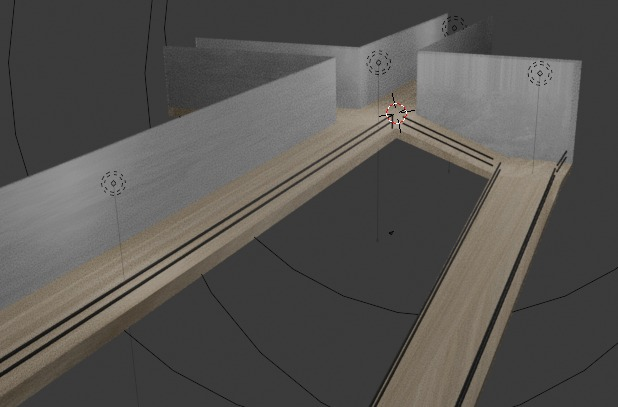
\includegraphics[width=16cm]{src/images/ThirdFloor.jpeg}
    \label{fig: Environment model}
\end{figure}

\subsection{Integration}

One of the primary challenges of this project was establishing effective integration between hardware emulation and the Gazebo simulation environment. To achieve this, ROS topics were chosen as the communication medium between the two systems, a decision driven by their modularity and compatibility with the Gazebo simulation.

On the other hand, there was no inherent support for ROS on the QEMU side, which required efforts to overcome this compatibility barrier.

\subsubsection{Adding ROS to QEMU}

One of the initial tasks in integrating ROS with QEMU was the difference in their native programming languages: ROS libraries are primarily written in C++ or Python, whereas QEMU is implemented in C.

To address this, it was necessary to find a C-based library capable of implementing a ROS node. After conducting research, the cROS library \cite{CROS_23} was identified as a suitable solution. This library provided the functionality needed to create ROS nodes in a C environment. However, integrating this library into QEMU's codebase presented an additional challenge.

To integrate the ROS library in C, all the library files were added to the repository and imported into the main QEMU file. This file, \texttt{vl.c}, contains the implementation of QEMU's main loop. That was made by including the header file \texttt{qom/cros.h}, which provides the implementation of the library and handles all the necessary internal includes. For more information about how the cROS works, it is possible to check the official manual \cite{cros_manual_24} or the source code \cite{CROS_23}.

The integration was achieved by introducing a dedicated thread within QEMU's main loop. This thread was responsible for running the ROS main loop, which linked to a TCP/IP socket to stablish communication with other nodes. Each node was assigned a callback function, responsible for publishing or subscribing to a topic, enabling interaction between QEMU and the broader ROS ecosystem. In the figure \ref{fig: ROS Implementation within STM32 QEMU}, it can be visualized.

\begin{figure}[h!]
    \caption{ROS Implementation within STM32 QEMU}
    \centering
    \includegraphics[width=12cm]{diagramas-qemu_ros_init.drawio.png}
    \label{fig: ROS Implementation within STM32 QEMU}
\end{figure}

Each callback from a sensor is responsible for reading a value from a ROS topic and writing it in the correct place in memory. For the topic from the motors, the value is read from the memory and it is written in the ROS topics. There is more  detailed information about it in the topic \ref{subsubsection: Complete integration}

The TCP/IP socket is important for making the correct link with the simulation because it connects the ROS provider from outside the QEMU with the ROS provider from inside QEMU. The initial idea of the TCP/IP socket can be visualized in the figure \ref{fig: QEMU with ROS socket initial idea}

\begin{figure}[h!]
    \caption{QEMU with ROS socket initial idea}
    \centering
    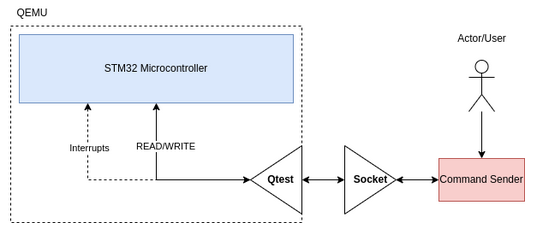
\includegraphics[width=16cm]{src/images/ros_socket.png}
    \label{fig: QEMU with ROS socket initial idea}
\end{figure}

In addition to the ROS main loop, it was necessary to add to the \texttt{run.sh} script, the TCP/IP socket configuration. With that, this script is able to compile the stm32\_qemu code, initialize the socket, select the binary code from the bluepill folder and execute the whole simulation.

\subsubsection{Complete integration}
\label{subsubsection: Complete integration}

\begin{figure}[h!]
    \caption{Emulation and Simulation complete integration}
    \centering
    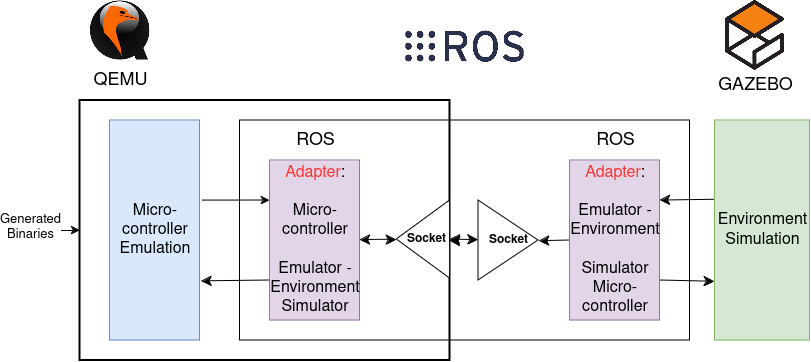
\includegraphics[width=16cm]{src/images/complete_integration.png}
    \label{fig: Emulation and Simulation complete integration}
\end{figure}

After integrating ROS into QEMU's emulation, it was possible to establish full communication between both systems. To achieve this, the following topics were defined:


\begin{itemize}
    \item \textbf{distance\_sensor\_(1-8)}: Topics responsible for sending the output of the distance sensors. These are published by the Gazebo simulation and subscribed to on the QEMU side.
    \item \textbf{encoder\_(left/right)}: Topics responsible for sending the encoder output. These are published by the Gazebo simulation and subscribed to on the QEMU side.
    \item \textbf{motor\_(left/right)}: Topics responsible for sending motor commands. These are published by QEMU and subscribed to on the Gazebo simulation side.
\end{itemize}

By running both environments with these topic references and establishing connections between the ROS nodes, the systems were able to communicate effectively— emulation sending commands to the simulation and the simulation providing sensor information, completing, finally, the system implementation. 

In the figure \ref{fig: General topics schema} it is possible to visualize all topics that have been published and subscribed to between the QEMU emulation and the Gazebo simulation. The arrows that are coming out of QEMU mean that it is the one that is publishing data there, and the arrows that are coming in QEMU mean that it has been reading. The same logic is applied to Gazebo.

\begin{figure}[h!]
    \centering
    \caption{General topics schema}
    \includegraphics[width=15cm]{diagramas-general_schema.drawio.png}
    \label{fig: General topics schema}
\end{figure}

Within the STM32 QEMU environment, each \textbf{distance\_sensor\_(1-8)} and \textbf{encoder\_(left/right)} has a topic subscription linked to a callback function. Whenever new data are received from the Gazebo simulation, the callback function is triggered, updating the memory location responsible for maintaining the GPIO input state.

For \textbf{motor\_(left/right)}, there are also callback functions. However, instead of writing data to the microcontroller's memory, it reads data from the location responsible for maintaining the GPIO output state. This data is then published on the respective motor topic. The code example \ref{lst:Callback function for motor 1 - From vl.c file} aims to illustrate the process in detail. The function is automatically executed every 100 milliseconds. 

\clearpage

\begin{lstlisting}[
    language=C++,
    caption={Callback function for motor 1 - From vl.c file},
    label={lst:Callback function for motor 1 - From vl.c file},
]
static CallbackResponse callback_motor_1(cRosMessage *message, void* data_context){
    char buf[1024];
    cRosMessageField *data_field;
    data_field = cRosMessageGetField(message, "data");
    uint32_t value, data;
    cpu_physical_memory_read(
        GPIOA_BASE_ADDR + 0x0c, 
        &data, 4
    );
    value = (data >> 1) & 0b111;
    ROS_INFO(
        node, "Right motor publish value: [%d]\n", 
        value
    );
    data_field->data.as_uint32 = value;

    cRosMessageSetFieldValueString(&data_field, buf);

    return 0;
}
\end{lstlisting}


In Figure \ref{fig: Callback Memory access example}, the flow of information can be visualized as it moves from the ROS topic to the microcontroller's memory for the \textbf{distance\_sensor\_(1-8)} and \textbf{encoder\_(left/right)} and, subsequently, from the microcontroller's memory back to the ROS topic for the \textbf{motor\_(left/right)}.

\begin{figure}[h!]
    \centering
    \caption{Callback memory access example}
    \includegraphics[width=16cm]{diagramas-uc_memery_read_write.drawio.png}
    \label{fig: Callback Memory access example}
\end{figure}


% \subsection{Communication between emulation and simulation}

% \subsection{}

\end{document}

